\section{Bedienungsanleitung und GUI}
\label{sec:frontend}

Im Folgenden wir die Installation und die Bedienung des Programmes erläutert, sowie der Aufbau der Oberfläche beschrieben. Das Programm kann unter \url{https://dev.spline.de/svn/CommonUnfold/trunk/} runtergeladen\footnote{\texttt{\$ svn checkout \url{https://dev.spline.de/svn/CommonUnfold/trunk/}}} werden. Im Ordner \texttt{src} muss die Datei \texttt{common\_unfolding\_draw.py} mit dem folgenden Befehl gestartet werden:\\

\centerline{\texttt{\$ python common\_unfolding\_draw.py\\}}


Wird das Programm gestartet, so befindet man sich im Startfenster (siehe~Abb.~\ref{fig:startFenster}). Über den Menüeintrag \texttt{File} können ersteinmal neue Schachteln erzeugt werden (\texttt{New By Surface, New By Dimension}) oder gespeicherte Arbeiten geöffnet werden (\texttt{Open File - Ctrl+O}).

\begin{figure}[htbp]
  \centering
  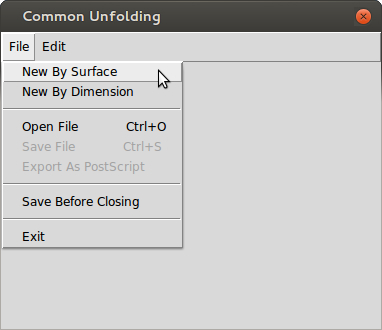
\includegraphics[scale=0.5]{03_pics/start.jpg}
  \caption{Startfenster}
  \label{fig:startFenster}
\end{figure}


%%%%%%%%%%%%%%%%%%%%%%%%%%%%%%%%%%%%%%%%%%%%%%%%%%%%%%%%%%%%%%%%%%%%%%%%%%%%%%%
%%%%%%%%%%%%%%%%%%%%%%%%%%%%%%%%%%%%%%%%%%%%%%%%%%%%%%%%%%%%%%%%%%%%%%%%%%%%%%%
%%%%%%%%%%%%%%%%%%%%%%%%%%%%%%%%%%%%%%%%%%%%%%%%%%%%%%%%%%%%%%%%%%%%%%%%%%%%%%%
% SCHACHTELN ERZEUGEN %%%%%%%%%%%%%%%%%%%%%%%%%%%%%%%%%%%%%%%%%%%%%%%%%%%%%%%%%
%%%%%%%%%%%%%%%%%%%%%%%%%%%%%%%%%%%%%%%%%%%%%%%%%%%%%%%%%%%%%%%%%%%%%%%%%%%%%%%
\subsection{Erzeugen von Schachteln}
\label{subsec:schachteln}

Die Anzahl der Schachteln kann man beim Erzeugen von neuen Schachteln frei wählen, \dH es können auch mehr als zwei Grundflächen ausgewählt werden. Aus dem sich ergebenden Commin-Unfold soll es möglich sein, die zuvor ausgewählten Schachteln zu falten. Bei der Erzeugung von neuen Schachteln, kann zwischen \texttt{New By Surface} und \texttt{New By Dimension} gewählt werden.

  \begin{description}
    \item [{New~By~Surface:}] Hier gibt man den Oberflächeninhalt an. Gibt es mehr als eine Schachtel, welche diesen Oberflächeninhalt hat, so werden diese erzeugt. Beispielsweise erzeugen die Oberflächeninhalte $22, 30, 34, 38, 40$ und $42$ jeweils zwei verschieden dimensionierte Schachteln, die Oberflächeninhalte $46, 54$ und $58$ jeweils drei Schachteln.
    \item [{New~By~Dimension:}] Hier gibt man die Breite, Höhe und Tiefe einer Schachtel an, alle weiteren, die in die gleiche Äquvalenzklasse fallen, werden erzeugt. Funktionierende Beispiele dafür sind die Dimensionen $1\times1\times5$, $1\times2\times3$ und $1\times4\times5$.
  \end{description}

Alle Schachteln werden in einer \emph{Preview} angezeigt und stehen zur Auswahl (Checkboxen) in einem neuen Fenster bereit (siehe~Abb.~\ref{fig:preview}). Man muss mindestens zwei Schachteln auswählen um das Programm zu starten. Existieren nur zwei Schachtel, werden diese automatisch Vorausgewählt. Zusätzlich kann man die Rotation der Schachteln in Grad angeben, diese werden dabei um ihren Urspungspunkt im Uhrzeigersinn rotiert.

\begin{figure}[htbp]
  \centering
  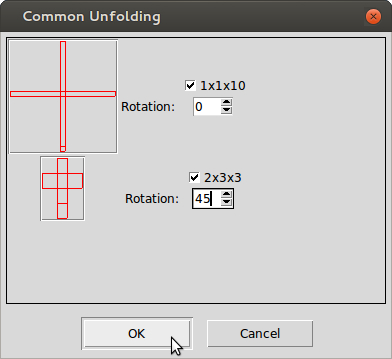
\includegraphics[scale=0.5]{03_pics/auswahl.jpg}
  \caption{Auswahlfenster für Schachteln}
  \label{fig:preview}
\end{figure}


%%%%%%%%%%%%%%%%%%%%%%%%%%%%%%%%%%%%%%%%%%%%%%%%%%%%%%%%%%%%%%%%%%%%%%%%%%%%%%%
%%%%%%%%%%%%%%%%%%%%%%%%%%%%%%%%%%%%%%%%%%%%%%%%%%%%%%%%%%%%%%%%%%%%%%%%%%%%%%%
%%%%%%%%%%%%%%%%%%%%%%%%%%%%%%%%%%%%%%%%%%%%%%%%%%%%%%%%%%%%%%%%%%%%%%%%%%%%%%%
% ZEICHENOBERFLÄCHE %%%%%%%%%%%%%%%%%%%%%%%%%%%%%%%%%%%%%%%%%%%%%%%%%%%%%%%%%%%
%%%%%%%%%%%%%%%%%%%%%%%%%%%%%%%%%%%%%%%%%%%%%%%%%%%%%%%%%%%%%%%%%%%%%%%%%%%%%%%
\subsection{Zeichenoberfläche und Startpunkte}
\label{subsec:zeichenoberflaeche}

Wählt man mehr als eine Schachtel aus und bestätigt die Auswahl mit \texttt{OK}, so gelangt man zur \emph{Zeichenoberfläche} (siehe~Abb.~\ref{fig:zeichenoberflaeche}).\\

Die Zeichenoberfläche besteht aus den folgenden vier Bereichen:

  \begin{description}
    \item [{(1)~Zeichenbereich:}] In diesem Bereich wird gezeichnet, hier     entsteht die neue Grundfläche aus der die links angezeigten Schachteln   gefaltet werden können.
    \item [(2)~Netze~der~Schachteln:] Im linken Bereich der Oberfläche werden alle ausgewählten Gitternetze untereinander angezeigt. Wir auf der Zeichenfläche gemalt so wird auf den Schachteln die ausgemalte Fläche angezeigt.
    \item [(3)~Startpunkte-Dialog:] Bevor man mit dem Zeichnen beginnt, können Startpunkte auf den einzelnen Schachteln gesetzt werden, dies kann in einem extra Fenster passieren (es wird beim Erstellen der Schachteln automatisch geöffnet), indem die genauen $(x,y)$-Werte für alle Schachteln eingegeben werden oder auch durch Klicken auf die Schachteln direkt im Bereich~(3). Das Setzen der Startpunkte kann auch über die Menüleiste \texttt{Edit $\rightarrow$ Set Start Points} erfolgen.
    \item [(4)~Werkzeugleiste] Hier können verschiedene Optionen bezüglich des Zeichenvorgangs eingestellt werden. Dazu gehören das Einstellen der Pinselgröße, Zeichenfarbe und Pinselform. Außerdem können die Optionen \texttt{Overwrite}, \texttt{Autofill} und \texttt{Continue} aktiviert werden. Diese Optionen werden im folgenden Abschnitt~\ref{subsec:zeichnen} erläutert.
  \end{description}

\begin{figure}[htbp]
  \centering
  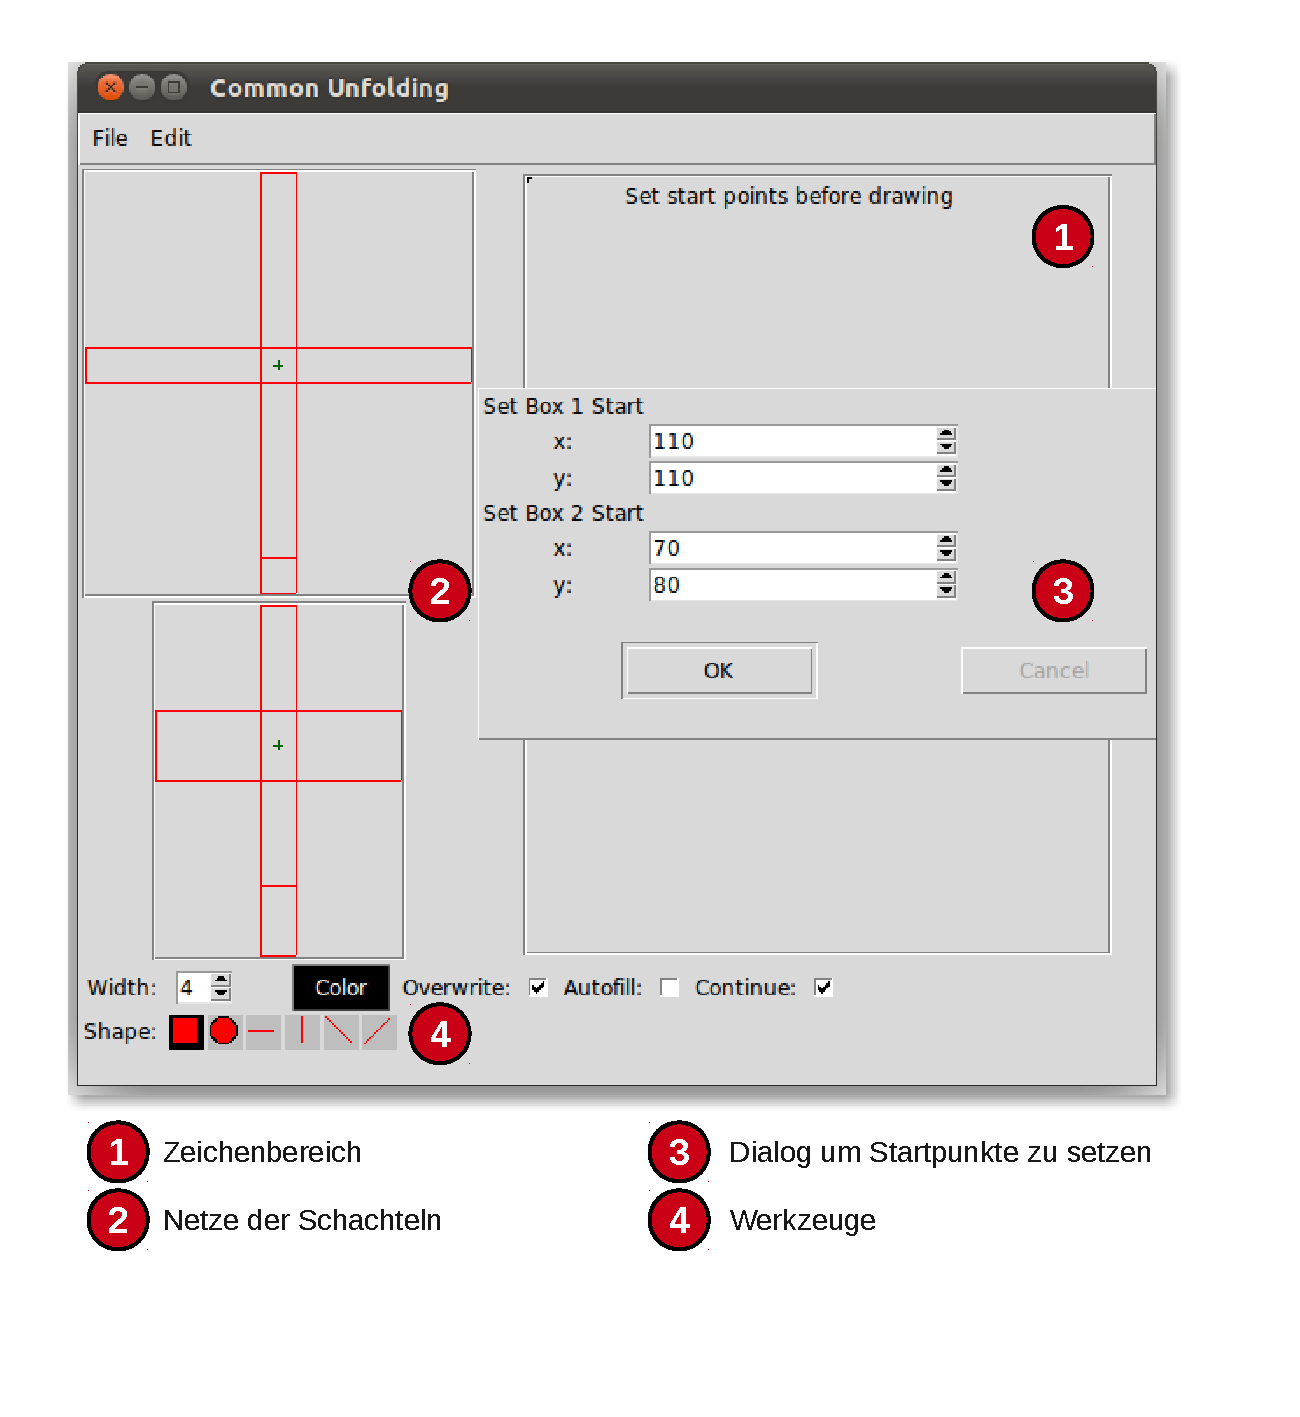
\includegraphics[scale=0.5]{03_pics/Zeichenbereich.pdf}
  \caption{Zeichenoberfläche}
  \label{fig:zeichenoberflaeche}
\end{figure}

%%%%%%%%%%%%%%%%%%%%%%%%%%%%%%%%%%%%%%%%%%%%%%%%%%%%%%%%%%%%%%%%%%%%%%%%%%%%%%%
%%%%%%%%%%%%%%%%%%%%%%%%%%%%%%%%%%%%%%%%%%%%%%%%%%%%%%%%%%%%%%%%%%%%%%%%%%%%%%%
%%%%%%%%%%%%%%%%%%%%%%%%%%%%%%%%%%%%%%%%%%%%%%%%%%%%%%%%%%%%%%%%%%%%%%%%%%%%%%%
% DAS ZEICHNEN %%%%%%%%%%%%%%%%%%%%%%%%%%%%%%%%%%%%%%%%%%%%%%%%%%%%%%%%%%%%%%%%
%%%%%%%%%%%%%%%%%%%%%%%%%%%%%%%%%%%%%%%%%%%%%%%%%%%%%%%%%%%%%%%%%%%%%%%%%%%%%%%
\subsection{Das Zeichnen}
\label{subsec:zeichnen}
Nachdem die Startpunkte gesetzt wurden, \bzw die Default-Werte übernommen wurden, kann im Zeichenbereich gezeichnet werden. Der erste Klick in den Zeichenbereich setzt den Ursprung des Tasters $(0,0)$. Zum Zeichnen klickt man einfach in den Zeichenbreich und hält die Maustaste gedrückt, der Curser wird zu einem Stift mit dem man malen kann. Gleichzeitig wird auf allen Oberflächen syncron gemalt, dies wird mit einem kleinen Kreuz auf den anderen Flächen angezeigt, wo sich der Curser gerade befindet (siehe Abb.~\ref{fig:zeichnen}). Es kann auch auf den Schachtelflächen gemalt werden. Die Fläche die im Zeichenbereich entsteht sollte zusammenhängend sein.

\begin{figure}[htbp]
  \centering
  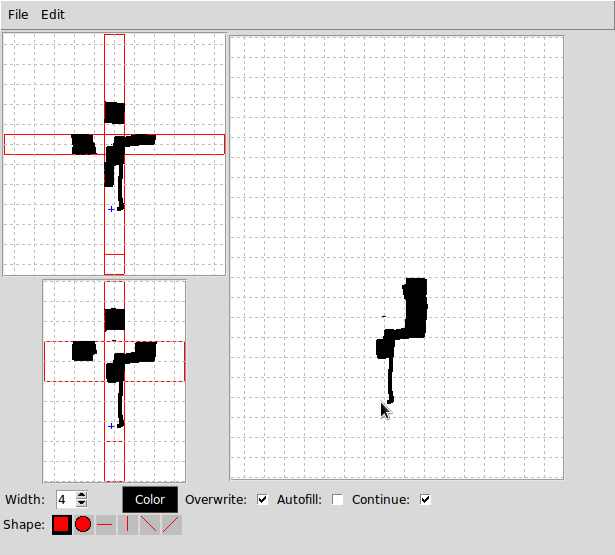
\includegraphics[scale=0.5]{03_pics/zeichnen.png}
  \caption{Zeichnen}
  \label{fig:zeichnen}
\end{figure}

Es können verschieden Optionen über die Werkzeugleiste eingestellt werden, diese werde im Folgenden näher erläutert.

\begin{description}
  \item [Overwrite] Aktiviert man \texttt{Overwrite} so werden breits ausgemalte Flächenstücke überschrieben.
  \item [Autofill] In Kombinationen mit dem aktivierten \texttt{Overwrite} bewirkt \texttt{Autofill}, dass durch \texttt{Overrite} entstandene unausgemalte Flächenstücke automatisch aufgefüllt werden.
  \item [Continue] [TODO:XXX:Was macht das denn?]
\end{description}




%%%%%%%%%%%%%%%%%%%%%%%%%%%%%%%%%%%%%%%%%%%%%%%%%%%%%%%%%%%%%%%%%%%%%%%%%%%%%%%
%%%%%%%%%%%%%%%%%%%%%%%%%%%%%%%%%%%%%%%%%%%%%%%%%%%%%%%%%%%%%%%%%%%%%%%%%%%%%%%
%%%%%%%%%%%%%%%%%%%%%%%%%%%%%%%%%%%%%%%%%%%%%%%%%%%%%%%%%%%%%%%%%%%%%%%%%%%%%%%
% LADEN, SPEICHERN, EXPORTIEREN %%%%%%%%%%%%%%%%%%%%%%%%%%%%%%%%%%%%%%%%%%%%%%%
%%%%%%%%%%%%%%%%%%%%%%%%%%%%%%%%%%%%%%%%%%%%%%%%%%%%%%%%%%%%%%%%%%%%%%%%%%%%%%%
\subsection{Menüleiste und Shortcuts}
\label{subsec:dateioperationen}

Über die Menüleiste können Dateien gespeichert, geladen und exportiert werden. Außerdem können Aktionen rückgängig gemacht und wiederholt werden, zudem kann die Option \texttt{Save Before Closing} aktiviert werden.

\begin{description}
  \item [Open File] Es können zuvor gespeicherte Dateien mit \texttt{Ctrl+O} geöffnet werden. Gespeicherte Dateien sind \texttt{CommonUnfoldFiles} mit einer Dateiendung \texttt{*.cuf}.
  \item [Save File] Dateien können als \texttt{*.cuf} gespeichert werden.
  \item [Export As PostScript] Dateien können ausschließlich als PostScript (\texttt{*.ps}) gespeichert werden. Gespeichert wird dann der Zeichenbereich (der Bereich auf der rechten Seite).
  \item [Save Before Closing] Diese Option kann aktiviert werden, so werden Dateien automatisch beim Schließen des Programms abgespeichert.
  \item [Undo] Mit \texttt{Ctrl+Z} können Schritte rückgängig gemacht werden.
  \item [Redo] Mit \texttt{Ctrl+Y} können Schritte wiederholt werden. 
\end{description}